%\documentclass[conference,final]{IEEEtran}
%\documentclass{sig-alt-full}
\documentclass{sig-alternate}

%\usepackage[pdftex]{graphicx}
\usepackage{graphicx}
% \usepackage{epsfig}
\usepackage{subfigure}
\usepackage[hypertex]{hyperref}
\usepackage{subfigure}  
\usepackage{color}
\usepackage{pdfsync}
% \usepackage{draftcopy}

\usepackage[small,it]{caption}

\usepackage{multirow}
\usepackage{ifpdf}

\long\def\comment#1{{ \bf \textcolor{magenta}{\bf #1}}}
\long\def\ccomment#1{{ \bf \textcolor{blue}{\bf #1 (SJ)}}}
\newcommand{\F}[1]{\B{\textcolor{red}{FIXME: #1}}}
\newcommand{\C}{\comment}
\newcommand{\CC}{\ccomment}
\newcommand{\fix}[1]{\textcolor{red}{\bf #1}}
\newcommand{\tc}{$T_c$ }
\newcommand{\tcnsp}{$T_c$}

\setlength\parskip{-0.15em}
\setlength\parsep{-0.0em}
\newcommand{\upup}{\vspace*{-0.6em}}
\newcommand{\upp}{\vspace*{-0.6em}}
\newcommand{\up}{\vspace*{-0.3em}}

\newif\ifdraft
%\drafttrue

\ifdraft
\newcommand{\fixme}[1]{ { \bf{ ***FIXME: #1 }} }
\newcommand{\jhanote}[1]{ {\textcolor{red} { ***Jha: #1 }}}
\newcommand{\yyenote}[1]{ {\textcolor{blue} { ***yye00: #1 }}}
\else
\newcommand{\jhanote}[1]{}
\newcommand{\yyenote}[1]{}
\newcommand{\fixme}[1]{}
\fi

\newcommand{\jitter}[1]{{$\sigma(\alpha)$}}

\newif\ifpdf
\ifx\pdfoutput\undefined
  \pdffalse
\else
  \ifnum\pdfoutput=1
    \pdftrue
  \else
    \pdffalse
  \fi
\fi

\ifpdf
\DeclareGraphicsExtensions{.pdf, .jpg}
\else
\DeclareGraphicsExtensions{.eps}
\fi

\begin{document}
\conferenceinfo{GMAC'09,} {June 15, 2009, Barcelona, Spain.} 
\CopyrightYear{2009}
\crdata{978-1-60558-578-9/09/06}

\title{Developing Autonomic Distributed Scientific
  Applications: A Case Study From History Matching Using Ensemble
  Kalman-Filters}
  
% \author{\authorblockN{Yaakoub El
%     Khamra\authorrefmark{1}\authorrefmark{2}, Shantenu
%     Jha\authorrefmark{2}\authorrefmark{3}\authorrefmark{4}},
%   \authorblockA{\authorrefmark{2} Center for Computation and
%     Technology, Louisiana State University, Baton Rouge, 70803}
%   \authorblockA{\authorrefmark{3} Department of Computer Science,
%     Louisiana State University, Baton Rouge, 70803}
%   \authorblockA{\authorrefmark{4} e-Science Institute, Edinburgh, UK}
%   \authorblockA{\authorrefmark{1} Texas Advanced Computing Center,
%     University of Texas, Austin, 78758} }

\numberofauthors{2}
\author{
\alignauthor
Shantenu Jha\\
       \affaddr{Center for Computation \& Technology,
          Louisiana State University, USA}\\
       \affaddr{Department of Computer Science,
          Louisiana State University, USA}\\
       \affaddr{e-Science Institute, University of Edinburgh, UK}\\
       \email{sjha@cct.lsu.edu}
\alignauthor
Yaakoub El Khamra\\
       \affaddr{Texas Advanced Computing Center,
          University of Texas Austin, USA}\\
       \affaddr{Center for Computation \& Technology,
          Louisiana State University, USA}\\
}

\maketitle
 \begin{abstract}
   The development of a simple effective distributed applications that
   can utilize multiple distributed resources remains challenging.
   Therefore, not surprisingly, it is difficult to implement advanced
   application characteristics -- such as autonomic behaviour for
   distributed applications. Notwithstanding, there exist a large
   class of applications which could benefit immensely with support
   for autonomic properties and behaviour.  For example, many
   applications have irregular and highly variable resource
   requirements which are very difficult to predict in advance.  As a
   consequence of irregular execution characteristics, dynamic resource
   requirements are difficult to predict a priori thus rendering
   static resource mapping techniques such as workflows ineffective;
   in general the resource utilization problem can be addressed more
   efficiently using autonomic approaches.  This paper discusses the
   design and development of a prototype framework that can support
   many of the requirements of Autonomic applications that desire to
   use Computational Grids.
   We provide here an initial description of the features and the
   architecture of the Lazarus framework developed using SAGA,
   integrate it with an Ensemble Kalman Filter application, and
   demonstrate the advantages -- performance and lower development
   cost, of the framework.  As proof of concept we deploy Lazarus on
   several different machines on the TeraGrid, and show the effective
   utilization of several heterogeneous resources and distinct
   performance enhancements that autonomics provides. Careful analysis
   provides insight into the primary reason underlying the performance
   improvements, namely a late-binding and an optimal choice of the
   configuration of resources selected.
 \end{abstract}

\category{J.2}{Computer Applications}{Physical Sciences and Engineering}
\keywords{Computational Science, Applications, Autonomics}
% \begin{keywords}
%    Distributed and Autonomic Applications, Distributed Application
%    Programming, SAGA
%  \end{keywords}

\section{Introduction}

Computational and Data Grids are an important component of the next
generation CyberInfrastructure to support scientific applications and
discovery.  They are characterised, amongst other properties, by
the following: dynamic, faulty and heterogeneous resources along with
error-prone services and applications.  To deal with the increasing
complexity of large-scale computing systems, computers and
applications must learn to manage themselves in accordance with
high-level guidance from humans -- a vision that has been referred to
as autonomic computing.

Designing and developing applications that can not only effectively withstand complex environments, but can actually exploit the value-addedness that arise from the collective capabilities are few and far in between. The reasons are complex and resist over-simplification; our work in this paper is motivated at demonstrating solutions that can be used to correct this limitation.

Not all autonomic behaviour have to be provided at the application
level or the system level, specially if mechanisms to implement
autonomic behaviour can be provided essentially at the application
level but without burdening the application developer.  In this paper,
we introduce Lazarus -- a framework that provides a general,
extensible approach for developing autonomic computational scientific
applications. Specifically, Lazarus provides the capability to use
different mechanisms to select resources based upon a strategy, enable
applications to be self-healing by providing fault-tolerance, the
ability to take advantage of autonomic behaviour as supported by a
wide range of information services. Lazarus provides a framework that
relieves the the application developer of the pressure and heavy
demands of providing a wide range of scientific application with
autonomic behaviour.  In general, we present SAGA as a programming
system to develop Autonomic Applications -- whether by directly
supporting Autonomic behaviour or via the development of frameworks
that provide autonomic behaviour.

% Autonomic or otherwise, have to be coded against.  Abstractions,
% such as frameworks can facilitate reuse.  Present SAGA as a
% programming system to develop Autonomic Application.  Provides
% generalized, extensible mechanisms for:


% Provides generalized, extensible mechanisms for:
% \begin{itemize}
% \item  Resource Selection
% \item  Placement
% \item  Fault Tolerance -- what are we going to say? Manual implementation
% \item Ability to plug-into decision support and Information Services
%   systems
% \item In general a framework can relieve the pressure/onus off the
%   application developer for a wide range of application
%\end{itemize}

% have definitely provided a massive increase in the computing power
% available for scientific applications, but this is due to the
% individual parts, and nothing to do with the sum of the parts, i.e.,

Grids are characterized by time-dependent resources loads, availability and access patterns; the aggregation of specialized resources in different administrative domains is one source of the heterogeneity.  Additionally, high-end Grid projects such as TeraGrid (TG) and DEISA have generally not enabled applications to be able to use distributed resources in a coupled or coordinated manner. The ability of applications to {\it scale-out} a critical requirement for distributed applications, has not been adequately developed or supported. % Grids have had limited success in engendering novel applications or usage modes.
Most applications and support-tools for distributed applications assume thatindividual ``jobs'' during the course of their execution will display a well-defined, static execution characteristics.  Thus not surprisingly most tools to address the dynamical nature of the Grids assume a fixed underlying resource requirement.  However there are class of applications for which the individual job run time characteristics are inherently difficult to predict and plan for. For these applications the resource requirement is dynamic and unpredictable; interestingly, the resource requirements and utilization might possibly be dependent upon both the execution trajectory and underlying infrastructure. Such applications are hard to develop and deploy. It is difficult to define a scheduling strategy that will be effective throughout the execution of a complete applications; hence static resource mapping is not an option.  It can be argued that the an optimal strategy for adapting to resource requirement changes is to provide application-level mechanisms that can respond dynamically if not autonomically.

% \yyenote{Feel free to move this, this is what I want to say about
%   Manish} \jhanote{this is perfect. thanks. its both technically
%   correct and strategically good} 

A key impediment to accelerated development of Grid applications and
consequently the uptake of Grids is the scarcity of high-level
application programming abstractions that bridge the gap between
existing grid middle-ware and application-level needs.  Application
developers are daunted by the complexity of the vast array of
low-level Grid and distributed computing software APIs that currently
exist; APIs have traditionally been developed using a bottom-up
approach that exposes the broadest possible functionality.  Coding
using these bottom-up APIs requires extremely verbose code to
implement even the simplest of application-level capabilities.  Many
Grid computing projects~\cite{realitygrid, gat, cog} recognized the
need for higher-level programming abstractions to simplify the use of
distributed computing for application developers.  The Simple API for
Grid Applications (SAGA) attempts to consolidate community effort and
make ends meet by employing a top-down approach to distributed
computing software infrastructure.  SAGA is the first comprehensive
attempt to provide a programmatic approach for the development of
applications so as to utilize distributed environments, either by
design or by virtue of deployment.  In addition to simplifying the
programming environment for application developers, SAGA insulates
applications from technological, version changes and other low-level
implementation details that regularly occur in the lower layers of the
software stack.

A motivation for this work is to understand how autonomic behaviour can be applied to Grids and Grid applications. We will understand which autonomic mechanisms are general, and thus can be encapsulated within a framework and which are accessed directly at the application-level. This is the first step in the direction of understanding how an autonomic framework can be developed that provides in a general, extensible way the ability to fulfill application level objectives such as improved throughput and lower time-to-solution. We will demonstrate the advantages of providing a general framework, such that it can be generalized to support a range of applications and multiple mechanisms for a given strategy. Underpinning the desire to develop such frameworks is the very tangible performance benefits that such abstractions provide.  Interestingly, we we will see in the Results section, this work also provides further confirmation of the ability of the right abstractions to enable the development of applications that can utilize the individual resources of the TG in a coupled and coordination fashion, and not just a single piece of big-iron.

% Aims of the paper are:
% \begin{itemize}
% \item Understand how Autonomic Behaviour can be applied to Grids
% \item Develop a general purpose framework \jhanote{Application
%     Objective: Improved Throughput and lower time to completion
%     Mechanism: Strategy: Resource Mapping and Resecheduling}
% \item Demonstrate advantages of extensible generalisable abstractions
% \item Specific application..\jhanote{A framework can support more than one strategy, but can also
%   support multiple mechanism for a given strategy.}
% \item Demonstrate performance advantages..
% \end{itemize}


We begin with a discussion of the application and
understanding of its characteristics, which will help motivate the
need for an autonomic framework. We should mention, this is certainly
is not the first time autonomic frameworks have been used to launch
and manage reservoir simulations. Bangerth~\cite{bangerth}, used an
autonomic framework to manage reservoir simulations for well-placement
optimization. At the moment, our work is focused on history matching
and reservoir characterization, however the next logical step is to
adapt Lazarus to run well/perforation placement studies. This might
lead to a convergence of SAGA and Accord~\cite{accord} in terms of
common functionality through different approach.

% The outline of the paper is as follows: In the next section we outline
% the scientific motivation and then describe the details of the
% components of the application that we have developed to use SAGA and
% Cactus.  \jhanote{to finish..}

% \jhanote{Possibly earlier and related work section?}

\section{Application: Description and Motivation} 

\subsection{Ensemble Kalman Filters: Scientific Motivation}

Ensemble Kalman filters (EnKF) are widely used in science and
engineering~\cite{DataAssim, KalmanPaper}. EnKF are recursive filters
that can be used to handle large, noisy data; the data can be the
results and parameters of ensembles of models that are sent through
the Kalman filter to obtain the true state of the data. The variation
in model parameters often has a direct and sizable influence on the
complexity of solving the underlying equations, thus varying the
required runtime of different models (thus the availability of the
results).  Varying parameters sometimes also lead to varying systems
of equations and entirely new scenarios. This obviously increases the
computational size requirements as well as memory requirements.  For
example as a consequence of the variation in size the underlying
matrix might become too large or even effectively doubling the number
of the system of equations, which could more than doubles the memory
required to solve the system of equations.

% The specific application that we investigate -- a prototype
% implementation of a 
The ensemble Kalman filter (EnKF) is a particularly interesting case
of irregular, hard-to-predict run time characteristics.  The forecast
model needs to run to completion which is defined as convergence to
within a certain value.  The run time of each model was unpredictable
and uncorrelated with the run-time of models running on the same
number of processors.  As at every stage, each model must converge,
before the next stage can begin, hence dynamically load-balancing so
as to ensure that all models complete as close to each other as
possible is the desired aim.  The number of stages that will be
required is not determined a priori. In the general case the number of
jobs required varies between stages.  Figure 1 shows a schematic of
the irregular and hard to predict run time characteristics of the
simulations.

\subsection{Ensemble Kalman Filters: Runtime Characteristics}

% Modern reservoir simulators  Reservoir flow modeling
% exists in the context of of the reservoir management function, a
% process that optimizes the interaction between data and decision
% making during the life cycle of a field.  One of the more popular
% popular models is the model that is used to solve for the
%Ensemble Parallel Kalman filters can be used for solving
%multi-component, multi-phase flow of fluids~\cite{AzizSettari, },
%atmospheric modelling~\cite{yaakoub_reference_add} and a whole other
%range of scientific and engineering
%problems~\cite{yaakoubreferenceadd}.  Typical input to such
%simulations of multi-phase flow in porous geometry consists of the
%initial conditions of both fluids (saturation, temperature, pressure,
%density etc.) as well environmental conditions (porosity,
%permeability, depth etc.)

%To ensure the fidelity of the such simulations for real models, data
%from simulations is validated against experimental data. This process
%is referred to as history matching. In this process, a large number of
%simulations with different parameters or initial data, are run and
%their results fitted against the experimental data. When simulation
%results vary from experimental data, the input parameters are modified
%to bring the model closer to the real experimental data. This process
%is repeated until a consistency criteria is observerd. The fitting
%method can be anything from a genetic algorithm, an ensemble Kalman
%filter or a simulated annealing process.  Each has its merits and
%drawbacks.  One of the best methods to perform such convergence
%criteria is the ensemble Kalman~\cite{needreferencehere} filter
%method, and it requires a hard synchronization point where it gathers
%all the data from all the various models and modifies model parameters
%to get better history matching in the iterations to follow.

% Typical reservoir simulations can vary in size from 100 grid points to
% tens of millions of grid points, and a decent model space can contain
% upwards of hundreds of models each with possibly varying size,
% physical model (i.e equations to solve) and more importantly different
% rock and fluid properties.  


%\subsubsection{Ensemble Kalman Filters: Stuff..} 

% Application Requirement $\rightarrow$ Resource Properties Resource
% Selection
% Adaptivity may arise due to the number of processors required by the
% many jobs being a variable, as well as the fact that the number of
% stages (ie involving global synchronization and subsequent
% distribution) is unknown {\it a priori}. There comes a point when
% providing the mechanism (logic and control) to the applications
% themselves to respond to these changes becomes more efficient and
% reliable than leaving it to a scheduler (or a meta-scheduler for that
% matter). We believe that this prototype application is well beyond the
% transition point and is a classic example of an adaptive application.
% The ability of a Cactus application to migrate to a more appropriate
% resources based upon network characteristics was demonstrated in
% Ref~\cite{escience07}.  We extend the sophistication of adaptivity to
% include: migration to better resource, based upon both compute and
% network characteristics, and choosing optimal resources to spawn to
% based upon local queue characteristics (as well as compute and network
% performance). The correct abstractions and programming approach
% enables the simple codification of an application that can determine
% best resource to migrate to based upon all of the above.

\begin{figure}
\begin{center}
\includegraphics*[scale=0.36,]{./figures/3StageKalmanFilter}
\end{center}
\up\up\up
\caption{Schematic illustrating the irregular execution or
  hard-to-predict run-time characteristics of a prototype
  implementation of an ensemble Kalman filter. The end-to-end
  application consists of several stages; in general at each stage the
  number of models generated varies. In the specific case studied in
  this paper, the size and granularity of the models varied within a
  stage. Consequently for any given stage the resource requirements
  varied from 8 processors to 64 processors.  The run time of each
  model was unpredictable and uncorrelated with the run-time of models
  on running on the same number of processors -- a truly independent
  variable. At every stage, each model must converge to within a
  specified value before the next stage can begin, hence dynamically
  load-balancing so as to ensure that all models complete as close to
  each other as possible is the desired aim.}
\label{fig:irregular_execution}
\up\up\up\up\up\up\up\up\up\up
\end{figure}

Even for relatively small input problem sizes at each stage, up to
several hundred models are generated which require from one to sixteen
processors to solve efficiently; the distribution of the number of
jobs and the run time-to-completion (\tcnsp) for a given processor count
varies by up to an order of magnitude.  Such hard to predict run-time
characteristics render static, data-flow independent scheduling
techniques difficult to use.  % We demonstrate how the use of
% appropriate programming abstractions like SAGA and Cactus enable the
% effective development of applications with non-trivial requirements,
% e.g., run-time resource selection based upon the application specific
% characteristics.

Hence a mechanism to assign models to available resources based on
their expected time to completion and resource requirement is useful.
Such a mechanism would estimate the time a model will spend in the
queue of a resource, the time it needs to run, and the time required
to migrate the data it requires/produces back and forth, and based on
that attempt to minimize the time required to perform each history
matching iteration.  In fact, with changing resource simulation
requirements (as is the case with models that find themselves lagging
behind the rest of the model pack), a mechanism which can take
advantage of of faster, cheaper or more powerful machines is even more
advantageous ~\cite{escience07}.

For example, once a model of application (as a job) has been mapped to
a resource, it is likely that the same model will have to be mapped to
another resource before the model reaches the desired convergence.
Thus for such applications, it is difficult to statically
(re-)schedule or manually control the execution of the jobs through
the application life-time.


\subsection{SAGA: Programming Systems and Abstractions}

% Our application consists of a exemplary distributed simulation that
% uses the added SAGA functionality to dynamically determine its ideal
% migration target based on ad-hoc and statistical network
% characteristics and to migrate itself in a heterogeneous Grid
% environment.  Although this a model application it can be easily
% adapted to more complex scientific applications.  Furthermore, our
% model application can be used as an autonomous benchmarking agent for
% Grid resources. In this section we briefly describe SAGA and the
% Cactus framework and discuss our motivation to use SAGA to incorporate
% high-level Grid functionality into Cactus.

\subsubsection{SAGA}

The Simple API for Grid Applications (SAGA) is an API standardization
effort within the Open Grid Forum (OGF)~\cite{ogf_web} an
international standards development body concerned primarily with
standards for distributed computing.  SAGA provides a simple,
POSIX-style API to the most common Grid functions at a sufficiently
high-level of abstraction so as to be able to be independent of the
diverse and dynamic Grid environments. The SAGA specification defines
interfaces for the most common Grid-programming functions grouped as a
set of functional packages (Figure 2).

%\up\up\up 
\begin{figure}[!ht]
  \begin{center}
      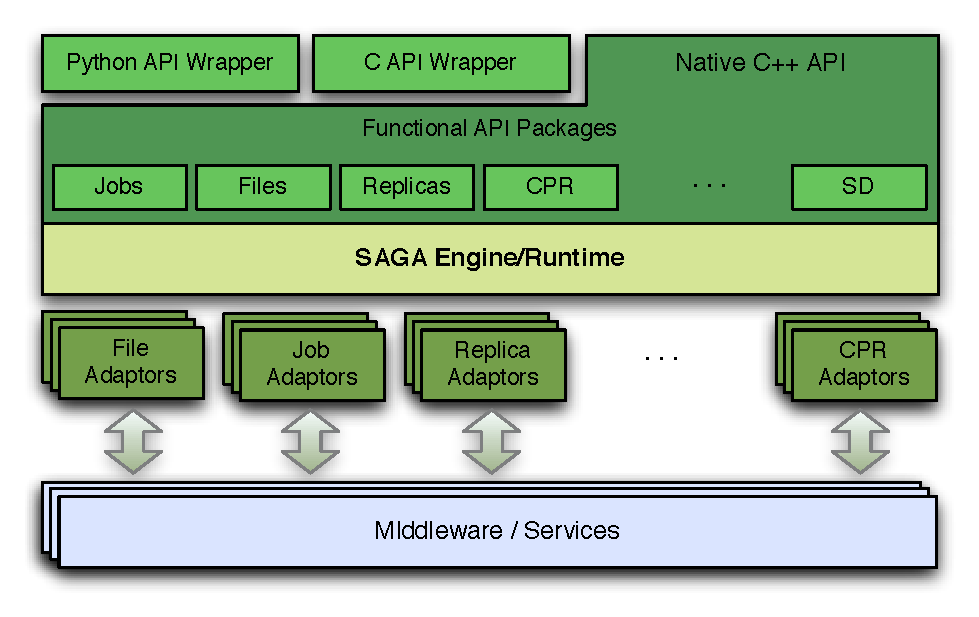
\includegraphics[width=0.40\textwidth]{stci_saga_figures-1.pdf}
  \end{center}
  \up\up\up\up\up\up
  \caption{\small Layered schematic of the different components
    of the SAGA landscape.  Middleware specific adaptors applications
    developed using SAGA make applications developed using SAGA grid
    portable.}\up\up\up\up\up\up
 \label{sagalayer}
\end{figure}

\begin{itemize}\addtolength{\itemsep}{-0.8\baselineskip}
\item File package - provides methods for accessing local and remote
  filesystems, browsing directories, moving, copying, and deleting
  files, setting access permissions, as well as zero-copy reading and
  writing
\item Replica package - provides methods for replica management such
  as browsing logical filesystems, moving, copying, deleting logical
  entries, adding and removing physical files from a logical file
  entry, and search logical files based on attribute sets.
\item Job package - provides methods for describing, submitting,
  monitoring, and controlling local and remote jobs. Many parts of
  this package were derived from the largely adopted
  DRMAA~\cite{drmaa_url} specification.
\item Stream package - provides methods for authenticated local and
  remote socket connections with hooks to support authorization and
  encryption schemes.
\item RPC package - is an implementation of the GGF Grid-RPC
  API~\cite{gridrpc_url} definition and provides methods for unified
  remote procedure calls.
\end{itemize}

The two critical aspects of SAGA are its {\it simplicity} of use and
the fact that it is well on the road to becoming a community {\it
  standard}.  It is important to note, that these two properties 
provide the added value of using SAGA for Grid application
development.  Simplicity arises from being able to limit the scope to
only the most common and important grid-functionality required by
applications.  There a major advantages arising from its simplicity
and imminent standardization.  Standardization represents the fact
that the interface is derived from a wide-range of applications using
a collaborative approach and the output of which is endorsed by the
broader community.

The SAGA C++ reference implementation~\cite{saga_web} was incorporated
into the Cactus Code Framework in Ref~\cite{escience07} to provide the
needed Grid programming functionality.  We believe this was an
important step in merging two programming abstractions to achieve an
effect that is greater that sum of the parts. 

{\it Developing Distributed Applications: } In the absence of a formal
theoretical taxonomy of distributed applications, we use 
Figure~\ref{sagaapps} as a guide.  Using this classification system,
roughly speaking, there are three types of distributed applications
(i) Applications where local functionality is swapped for distributed
functionality, or where distributed execution models are provided;
(ii) Applications that are developed using well known patterns, for
example MapReduce, which in turn is implemented using SAGA; (iii)
Finally, applications based upon frameworks that are developed using
SAGA. These frameworks support specific application-level and system
functionality and can be used by multiple applications (hence a
framework and not an application-level solution).  SAGA has been used
to develop system-level tools and applications from each of the three
different types.
\begin{figure}[!ht]
  \begin{center}
%\up\up\up\up\up\up\up\up\up\up\up\up\up
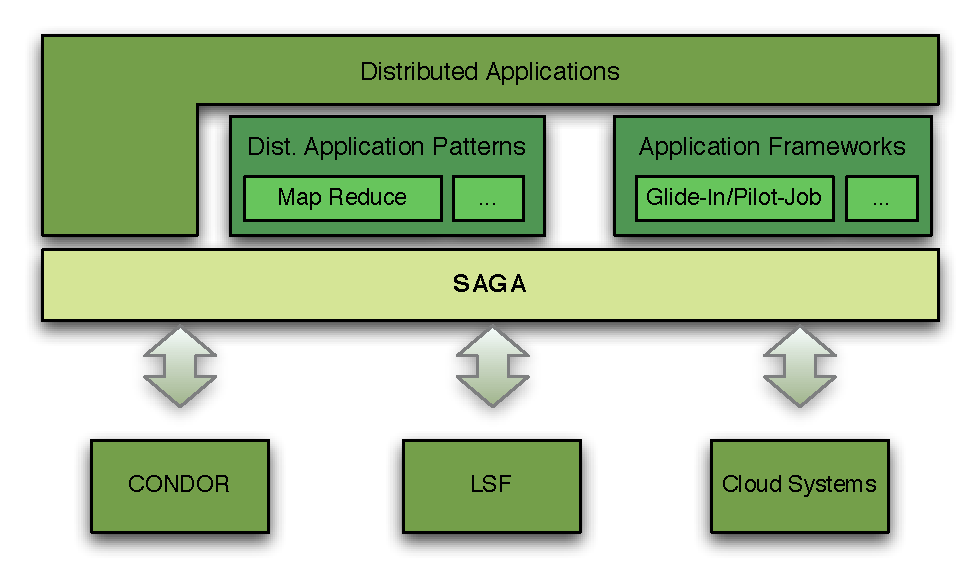
\includegraphics[width=0.43\textwidth]{saga_platform_figures.pdf}
\end{center}
  \caption{\small(Right) Schematic showing the different ways in which
    SAGA can be used to develop distributed applications}
 \label{sagaapps}
\end{figure} %
Figure~\ref{fig:abstractions} summarizes the abstractions developed
and used in this work to support the clustering of sub-jobs into a
larger big-jobs and the effective dispatching of the sub-jobs.  The
specific capability to cluster sub-jobs, is provided to the
application via the \emph{BigJob} abstraction. This abstraction
enhances the SAGA job model with the capability to allocate larger
chunks of resource for a single job.  
\begin{figure}[t]
      \centering
      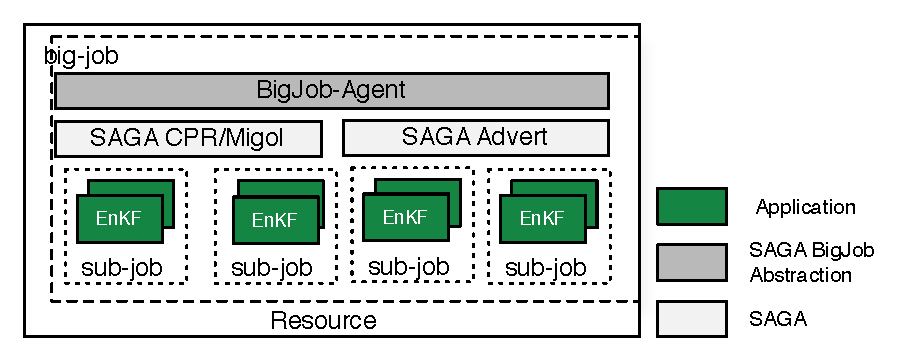
\includegraphics[width=0.430\textwidth]{./figures/enkf_bigjob.pdf}
      \caption{\footnotesize The {\it BigJob} abstraction for simulations of
        biological systems, but has been generalized and extended to
        the History Matching problem. Specifically the BigJob
        abstractions has been added with fault-tolerance capability
        and the ability to effectively place the BigJob using
        autonomic information. These capabilities form the basis of
        the Lazarus autonomic framework for computational science
        applications.}
      \label{fig:abstractions}\up\up\up \up\up\up
\end{figure}

{\it SAGA: BigJob Abstraction:} A common system-level abstraction is
the support for Glide-In jobs, which represent a placeholder for a
set of sub-tasks (see Ref.~\cite{saga_royalsoc}).  For a Glide-In
job, a sufficiently large chunk of resources is requested. Smaller
sub-tasks can then rapidly be executed through the Glide-In job.
%Figure~\ref{fig:remdmanager_v11} summarizes the abstractions used
%within the RE framework. 
The SAGA Glide-In abstraction is used to support the commonly
occurring requirement to schedule multiple sub-tasks relative to each
other and not in competition with other jobs submitted to the batch
queue system.  Thus, a \texttt{big\_job} and \texttt{sub\_job} object
are defined; for each \texttt{big\_job} object, a Glide-In job with
the desired number of resources is started, and \texttt{sub\_job}
objects -- which correspond to individual replicas, are mapped to a
\texttt{big\_job} using the jobid as reference. It is helpful to
reiterate that although there is a big\_job object, it is submitted as
a Glide-In job, and that BigJob abstraction in turn utilises the
Glide-In abstraction to map the individual big-job and sub-jobs to
physical resources.  Details of the \emph{BigJob} abstraction can be
found in Ref.~\cite{saga_royalsoc}.

By using the BigJob abstraction, Lazarus enables using multiple-resources, using application-level scheduling applied dynamically, i.e., mapping the sub-tasks requirement to the resources available at the instant the sub-tasks become available and ready to run, as opposed to {\it a priori} static method of job submission.  In other words, an advantage of the Lazarus framework (currently based upon the BigJob abstraction but soon to use the Framework for Adaptive and Ubiquitous Scalable Tasks (FAUST)~\cite{faust_url}) is the flexibility it provides -- which can be referred to either as late binding or loose-coupling between application resource requirement and resource assignment.

{\it Developing Applications using SAGA and Cactus:} Cactus provides
the support and features required to implement adaptivity e.g.,
checkpoint, restart and migrate thorns. SAGA provides the ability to
implement these features in a specific distributed environment, for
example, move files from location A to location B, start a job on
resource X from resource Y.  Thus the two programming abstractions
that Cactus and SAGA provide are natural complements of each other.
As alluded to, we do so by interfacing SAGA with Cactus and thus are
able to draw on the many advantages of using SAGA function calls from
within a Cactus application.  The result is an application that uses
these two important application-level frameworks and abstractions to
create a truly distributed application.  SAGA provides the capability
for the the distributed aspects. SAGA provides a high-level
programming interface to Grid functionality. By utilizing the
advantages of proper programming abstractions, by integrating SAGA and
Cactus and demonstrate the usefulness for Grid application development

\up\up
\subsection{Autonomic Resource Selection at Runtime Using Batch Queue
  Predictor}
Batch Queue Predictor~\cite{bqp, bqp_url} (BQP) is a tool that is
available on a number of TG resources that allows users to make
bound predictions of how much time a job of a giving size and duration
will spend in the queue.  BQP is traditionally used for determining
the status of the queue resources available and static resource
mapping. This prediction is given with a degree of confidence
(probability) that the job will start before a certain deadline
(i.e. the time in the queue) and quantile. Quantile value is a measure
of repeatability; more precisely it is an indication of the
probability that jobs of similar sizes and durations will have the
same wait time. This information is vital when submitting jobs to
various machines as the longer a job sits in the queue, the longer the
delay for the entire stage.

What is enticing about BQP is that it provides information that is of
importance to the class of applications that we are interested in,
namely, the ability to predict with given probability which resource
and when a job (with a specified number of processors and estimated
run-time) is most likely to finish.  This is typically harder to
predict correctly than which resource a job with specified
characteristics is most likely to run first.  The application uses BQP
internally within an application to make resource selection decisions
dynamically (at run-time, as opposed to static queries) and
automatically (the logic of how to process BQP information is embedded
in the application).

For our application we use the BQP command line tools, that are called
through a python wrapper from the Lazarus.  For a given resource list,
the python wrapper around the BQP executable finds the resource and
queue where if submitted, a BigJob of a given size and expected run
time, will have a good chance (or high confidence) of getting through
the queue and start running the earliest. Confidence is the
probability that the job will run within the specified deadline; to
obtain a confidence of 1.0, an impractically high queue time would be
required. For our applications, not knowing the granularity of the
available BQP data, we opted to use a confidence of 0.75 (and the
default value of quantile to be 0.75.)  The choice of 0.75 is a
justified good first approximation -- as the bias in our results due
to the choice of confidence to be 0.75 is minimal. We will elaborate
on this in the Challenges section.

% e did simple experiments to the test the dependence on the confidence
% and quantile values; we find that the output is not very sensitive to
% the confidence
% are logical but require a more detailed sensitivity
% analysis for completeness.

% \jhanote{Need to say, what the requirements are, establish very
%   quickly why autonomics is the solution to the specific problem and
%   then talk about the solution -- first the primitive (ie scripts)
%   then the Lazarus (using BigJob and BQP).}
% \yyenote{Addressed, please have a look}  

\section{Lazarus: Motivation, Architecture and Control Flow}

% \subsection{Lazarus}

To reliably launch hundreds of reservoir simulations and collect the
data they produce repeatedly across different machines, we needed a
fast, easy to use abstraction, this lead to the use of BigJob
abstraction~\cite{saga_royalsoc}.  Lazarus builds upon earlier work,
and extends the BigJob abstraction to explicitly utilize autonomic
decision making based upon BQP as well as support for
fault-tolerance. This is the basis of the general purpose autonomic
framework Lazarus.

After losing many jobs to various errors such as running out of allocated diskspace, hardware failure and file-copy failure, we quickly came to the conclusion that autonomy and self healing are important features that we needed to incorporate in Lazarus to ensure all large scale history matching runs complete successfully. With fault tolerance, we no longer wasted thousands of Service Units (SU) running simulations with missing/corrupt ensemble members, as they are resurrected.  On the other hand, the autonomy incorporated in Lazarus, while basic, ensures that we optimize the job sizes to have a higher chance of getting through the queue without delay.

For the current implementation, we started off using simple, portable
python scripts -- based upon SAGA, that handles job-launching and data
migration. % This makes Lazarus a modular, scalable and extensible
% framework for autonomic applications based upon the SAGA programming
% system.  
Lazarus uses the BigJob abstraction to launch simulations,
the SAGA file adaptor python bindings to move files from one machine
to another and BQP data from a small python wrapper around the BQP
command line tool to retrieve the optimal location and number of
BigJobs required to satisfy the computation power required (Figure 5).

Lazarus's healing ability depends on user-defined tests on the data to
make sure it is not corrupt, missing, or otherwise defective. If a
simulation is found to be defective it is resubmitted to be run
again. This self resurrection ability overcomes some of the
catastrophic errors encountered when running large numbers of jobs
such exceeding wall clock time, running out of diskspace (resubmit on
a different machine) and of course node failure.

\begin{figure}
\begin{center}
%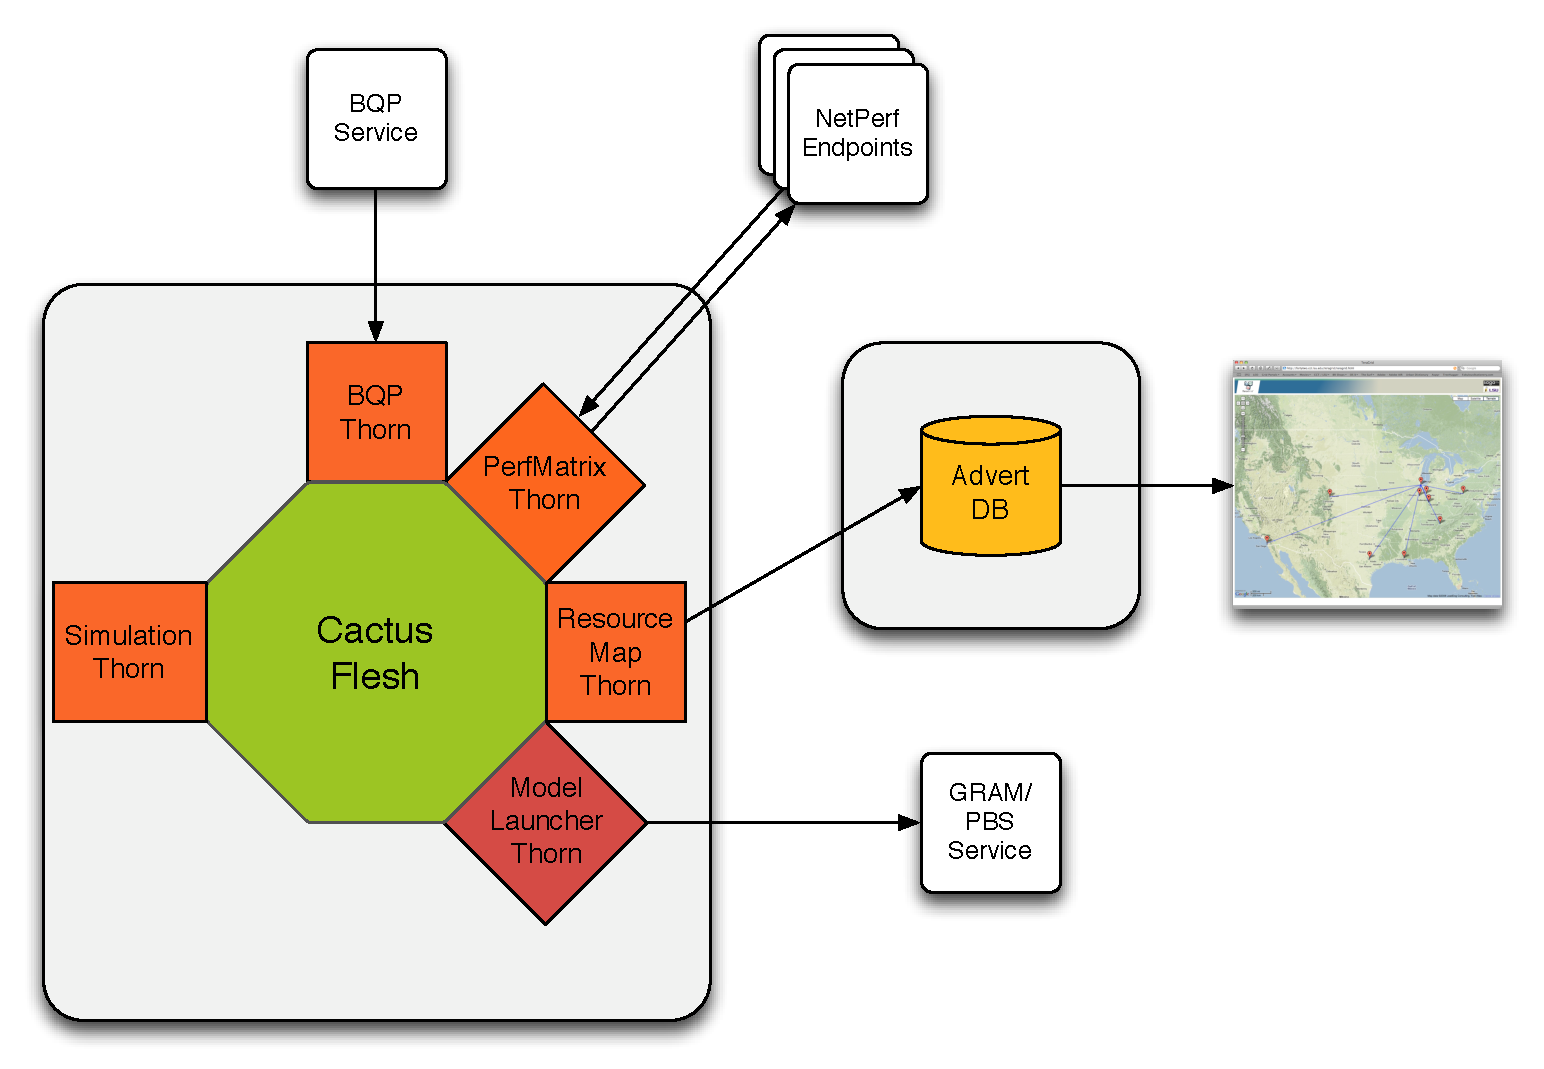
\includegraphics[scale=0.34]{./figures/ApplicationArchitecture}
%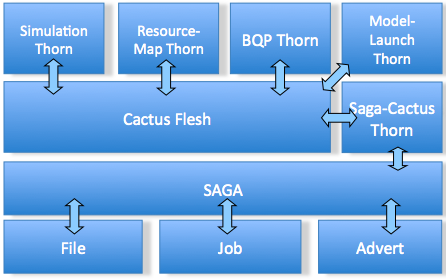
\includegraphics[scale=0.34]{./figures/kalmanfilterlayer.png}
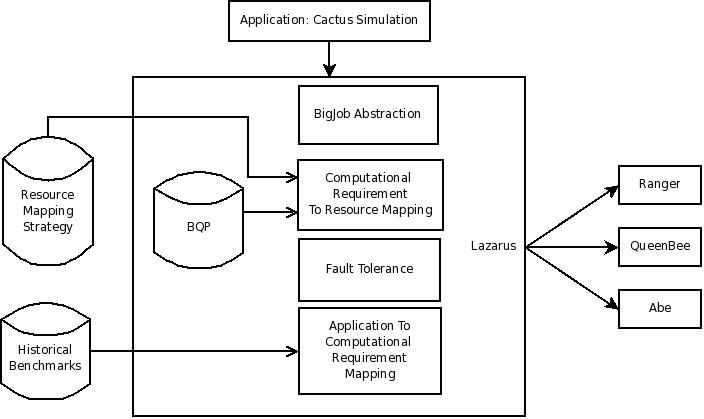
\includegraphics[scale=0.4]{./figures/Lazarus_01.jpeg}
\end{center}
\caption{Architecture of Lazarus -- a Framework for Developing
  Autonomic Computational Science Applications. The ``Resource
  Mapping'' Strategy input is provided by BQP. Given the size of the
  individual tasks, the ``Historial Benchmarks'' help determine the
  size of the sub-jobs. (For the specific workload chosen, it so
  happens that the size of each sub-job is 16).}\up\up\up \up\up\up
\label{fig:application_architecture}
\end{figure}


\subsection{Autonomy}
The Lazarus framework contains several aspects of autonomy: it has
self-configuration (deployment on resources), self optimization (using
BQP data), self monitoring (checking its own output) and of course
self healing (resubmission of faulty simulations). These aspects have
been implemented with varying level of intelligence: the self
optimization for example is a basic algorithm that uses BQP data to
assign big-jobs to resources, but does not take into consideration
bandwidth requirement and the cost of copying files across
machines. The self-healing on another hand can typically resurrect
jobs that fail due to node failure as opposed to software
failure. Many autonomic features of Lazarus will find their way into
the FAUST framework, where they will be improved to incorporate
sophisticated inherent intelligence.  

It is also worth mentioning the due to the correct programming
abstractions, we did not have to develop most of the tuning
mechanisms, but were able to write suitable interfaces to these
mechanisms.


\subsection{Failure Modes}
As early as the first non-trivial Lazarus run we encountered failures. They
varied in nature (hardware/environment) and severity. As Lazarus progressively
used more resources, many more failure modes were encountered.
Many were errors that are irrecoverable and resulted in a
cold restart from scratch; others were recoverable with a simple simulation 
result-check fault tolerant component built into Lazarus.

Representative hardware failures encountered:
\begin{itemize}\addtolength{\itemsep}{-0.8\baselineskip}
\item{Lost a compute node from the pool}
\item{Lost a network connection to a machine, BQP or the advert service}
\item{Could not write to /scratch because it was taken down for maintenance}
\end{itemize}
Amongst the modes of failure, we found that we reliably recover from node failure and failure to write data to disk, but not network failure. The status of any given job is reported in a one-way poll for current state.  We will discuss how to overcome such limitations using the "heart-beat" monitor (in FAUST) in section VI.

Representative software environment failures encountered:
\begin{itemize}\addtolength{\itemsep}{-0.8\baselineskip}
\item{Missing or wrong shared libraries}
\item{Wrong or inadequate environment variables}
\item{Run out of quota on disk, wrote too many files to the same directory}
\item{Run out of SU's in the allocation}
\item{No internet connection to the compute nodes (no BQP, no advert service)}
\item{MPI error that causes a simulation to stall (this happened because of a faulty installation and was corrected)}
\end{itemize}
In software environment failures, typically jobs terminate with errors
or are killed, before the simulations results are written to
disk. Unsurprisingly we ran into all of these failures while
developing Lazarus, and were able to recover from all of them except
for the network connectivity in the compute nodes, as this would
register the job's state as "unknown". This would be solved with the
aforementioned heart-beat monitoring system.

Representative simulation failures encountered:
\begin{itemize}\addtolength{\itemsep}{-0.8\baselineskip}
\item{Missing parameter files or executable}
\item{Wrong parameter files, or erroneous setup of parameter files}
\item{Divergence in the solver, causing NaN shuffling and leading to exceeding the requested wall clock time}
\item{Under-estimation of the required wall clock time}
\item{Hitting /scratch or /home too often (because of checkpointing), leading to very low access speeds and exceeding the requested wall clock time}
\end{itemize}
Some of the simulation failures are relatively easy to guard against,
namely the wrong parameter file or missing executable. The other
errors are harder to detect and rectify.

To facilitate deployment we use python bindings to the SAGA-based
BigJob abstraction. Using these scripts, a user-specified number of
stages each containing a user-defined number of models can be launched
to the grid. As the models of a given stage run to completion, a
second set of error-checking jobs are launched that ensure all the
models ran to completion before the Kalman gain calculation is
performed. This error-checking mechanism attempts to re-submit the
failed jobs, and if met with failure a second time, the stage is
halted to allow for user intervention.

\subsection{Fault Tolerance}
Given the many, different failure modes, it is only natural to support
fault-tolerance so as to provide Lazarus with built in self-healing
capabilities. These capabilities rely on a tool-check/calibration test
and output file checks. After simulations have finished and their
output files are copied, Lazarus proceeds to perform a tool-check
on a sane file. The purpose of the tool-check is to make sure the
tools that will be used in checking the output files from the
simulations are available and behave according to expectations. Once
the tools are verified, they are used to check the output of all the
simulations. If a simulation is found to have missing, incomplete or
otherwise faulty output, it is flagged for resubmission.  After all
output is checked, the faulty simulations are resubmitted and upon
termination, all output is checked again and upon success, Lazarus
proceeds.


\subsection{Simulation Components}
\begin{figure}
\begin{center}
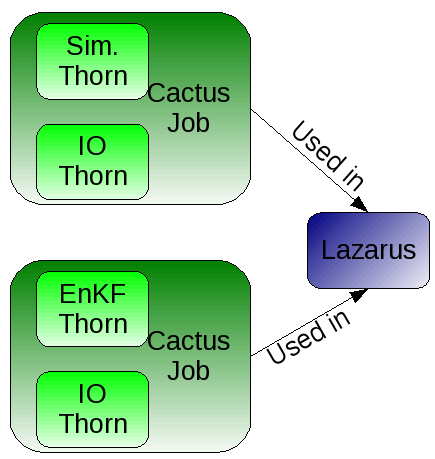
\includegraphics[scale=0.5]{./figures/Simulations.png}
\caption{Schematic diagram illustrating the different simulation components, and and that the application (a Cactus-based Reservoir
  simulation) utilizes Lazarus.}\label{fig:application_usage} 
\up\up\up \up\up\up \up\up\up \up\up\up \up\up
\end{center} 
\end{figure}
 
The simulation component in the Lazarus framework is based on the Cactus framework and employs two Cactus builds: a reservoir simulation build that uses the reservoir simulation thorns and an EnKF build that uses the EnKF thorns. Both builds use the Cactus IO thorns and functionality from third party libraries such as PETSc~\cite{PETSc} and HDF5 (see Figure ~\ref{fig:application_usage}).


The reservoir simulation thorn solves a system of non-linear partial
differential equations for compressible multiphase flow through porous
media. The simulator is in effect a black-oil reservoir simulator that
uses the implicit-pressure, explicit-saturation formulation and a
finite difference discretization. The system of equations is solved
using a Krylov subspace solver using PETSc. For a prototype
implementation we chose a multiphase, multicomponent fluid flow
through porous media simulator.
%and implemented it in the Simulation thorn in Cactus.

The EnKF thorn is an ensemble Kalman filter thorn that requires, as input, the state vectors of the various ensembles at regular intervals. These are effectively the checkpoint files of the simulations (forecasts) in addition to their production data. Once the EnKF has all the state vectors from all the ensembles, it performs the analysis and a new set of ensembles with now modified state vectors need to be run. This process is repeated until there are is no more historical data to match against. Typically, production history is averaged on a monthly basis, sometimes on weekly or even daily basis, over a period of a few years. For this reason, a typical production run will involve hundreds of stages.

\subsection{Lazarus Components}

The various components that are utilized by Lazarus are shown in Fig.~\ref{fig:application_architecture}.  As mentioned earlier, Lazarus in its current incarnation is a set of small, fast, portable and modular interfaces. These interfaces make extensive use of high level abstractions such as BigJob and SAGA.

\begin{figure} 
  \begin{center} 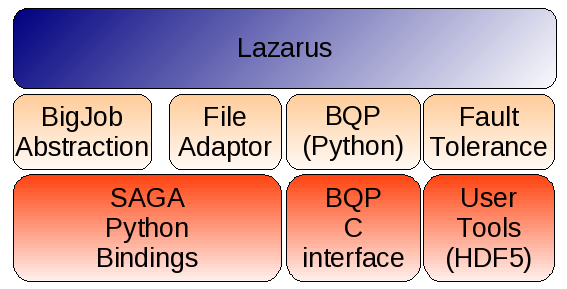
\includegraphics[scale=0.5]{./figures/Architecture.png} \caption{Block diagrams outlining how Lazarus relates to other SAGA components. Lazarus is built on several components: BigJob abstraction, SAGA file adaptor, BQP python wrappers and fault tolerance functions that are based on SAGA python bindings, BQP command line tools and HDF5 tools respectively.}\label{fig:application_architecture}
\up\up\up\up\up\up\up%\up\up\up\up\up
\end{center}
\end{figure}
 
For runs distributed across several machines, Lazarus needs to gather the data from all different machines into one location where the EnKF can run. To that end, the python bindings to the SAGA file adaptors are used to copy files over to the resource where the EnKF will run, and copied back to all other resources after the analysis stage. Since we are not working with a large scale production history matching run, the amount of data transfer involved does not impose any noticeable performance issues. Naturally, investigating the optimal location for placing the EnKF application, based upon network performance and real-time performance as discussed in Ref.~\cite{escience07}, will find its way into the next iteration of Lazarus implementation.

Lazarus also uses non-SAGA components, such as a small python wrapper
for BQP. This allows Lazarus, namely its resource management function,
to query BQP for the ``optimal'' job size and duration for any given
resource. Lazarus also uses a user specified check for the integrity
of the simulation data. In our case, this is done through various
system and HDF5 calls to make sure the files exist, are not sized
zero, and a user specified command using HDF5 tools (h5ls) returns
successfully (Figure 7).

Lazarus is distinct to other well established and successful approaches such as Accord~\cite{accord} for autonomic computing, in that it is not a component-based programming system but it is a framework already composed of multiple components. Importantly the programming system that is used is SAGA -- both for the application and the Lazarus framework.

\up\up\up
\subsection{Control Flow}

\begin{figure}
\begin{center}
 %  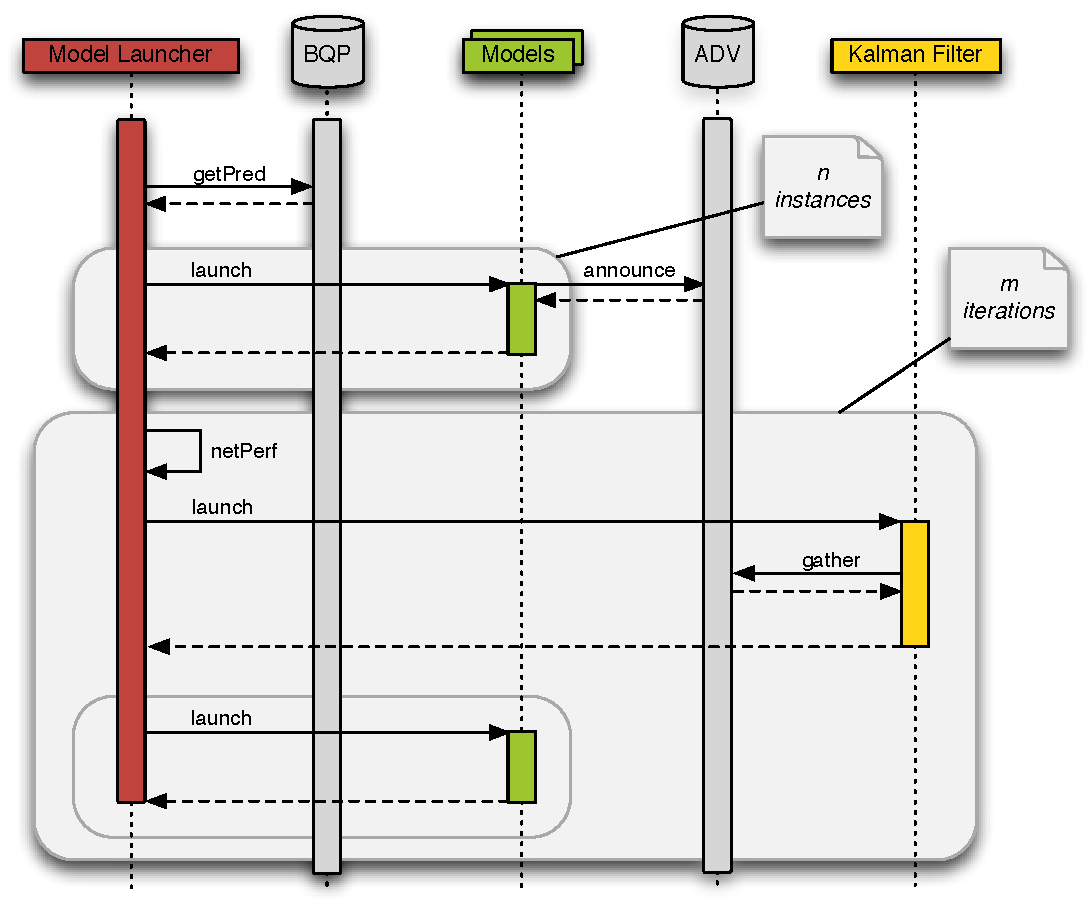
\includegraphics[scale=0.5]{./figures/SequenceDiagram}
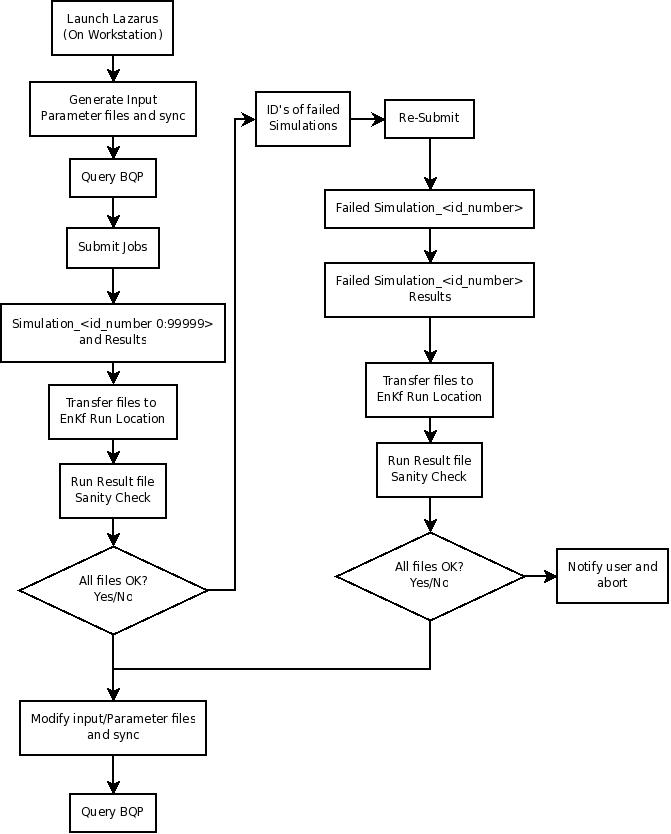
\includegraphics[scale=0.35]{./figures/Diagram1.jpeg}
\end{center}
\caption{A high-level overview of the control flow of an application using Lazarus}
\up\up\up \up\up\up \up
\label{fig:controlflow}
\end{figure}

%The application starts by getting BQP data for a list of candidate
%machines, assigns simulations to machines and submits the jobs to the
%respective machine scheduler. Once all the simulations are submitted,
%the history matching application (in our case a Kalman filter) is
%submitted to run. The Kalman filter application is run on the
%machine that will run 50\% or more of the entire simulations or the
%machine that has the highest bandwidth amongst the machines used for
%the simulations.  Once the simulations start, they notify the advert
%service of their starting time and location; upon successful
%completion, they also notify the advert service of the path of the
%files they output.  Meanwhile the history matching application is
%notified of the completion of the simulations and modifies the models
%used in the reservoir simulation. The modified models are then
%submitted again as a second stage and the entire processes is
%repeated.

% \jhanote{Mapping: Need discussion on the two-levels of decision
%   making. I thought we had done this!}  {\it Mapping of physical-model
%   requirements into compute-resource requirements} {\it Mapping
%   compute-resource requirements into available resources}

To prepare for launching Lazarus, a model generator is required to
create the initial data (initial state vectors) for all the
ensembles. This is typically done a priori to running Lazarus, and
performed on one resource then synchronized against all others to
ensure consistency.

Before launching Lazarus, some input parameters need to be specified.
These are the executable names, working root directory, simulation
directories, number of simulations per stage, number of stages, simulation
size and so on. The current implementation supports varying simulation
sizes across a single stage and from stage to stage. At
the moment, we use a constant size of 16 cores per subjob for all machines
for simplicity, as the load-varying, adaptive mesh
refinement reservoir simulator is still under development.

Given the number of jobs per stage, and historical benchmark
information on various machines, an estimate for the total SUs
required is computed and sent to the Lazarus resource manager. The
resource manager queries BQP for the optimal sizes and durations and
creates a list of BigJobs, their sizes, durations and the
resource/queue where they will be submitted. If we have more than one
resource available, the SU requirement is satisfied based on a
round-robin algorithm, iterating over resources and adding BigJobs
until no more BigJobs need to be submitted.

Once the resource list is formulated, Lazarus uses the BigJob
abstraction to submit jobs to all BigJobs in the resource list. The
status of the jobs and BigJobs is reported on regular intervals
through a logging mechanism. Upon completion of all the subjobs,
Lazarus performs a calibration test where it runs the user-specified
output-check on a pre-validated file, to ensure all the tools are in
place and in working order. It then proceeds to check the output from
all simulations to ensure sanity of output. Simulations that have
faulty output are then collected into a list and resubmitted. The
output is again checked for sanity: if all is well we proceed with the
EnKF run (i.e. the analysis) and if not Lazarus will abort with a
detailed log file of the error. This is mainly to safeguard against
wasting SUs on corrupt runs. Once the analysis is complete, Lazarus
repeats the forecast iteration with the newly modified state vectors
and the history matching continue (Figure 8).

% For the problem size studied, the sub-tasks required mostly less
% than 32 processors. For this paper we used the earlier developed
% frameworks and deployed it on a single large machine -- NCSA's
% Abe. A mechanism (multiple, distributed versus single machine) that
% is more efficient for physical models with sub-tasks that have
% typically low processor counts, will not necessarily be the more
% efficient as the typical sub-task size increases. Therefore it is
% crucial that any general-purpose solution be usable on both single
% large machines to multiple machines.  We can enhance throughput
% further by applying the Glide-In mechanisms discussed in the earlier
% section, which facilitate dynamic tasks being aggregated from
% similar sub-tasks. We will report on the results of this and whether
% the framework can be used on high-end petascale supercomputers in
% future work.

\section{Experiments: Results and Discussion}

In this section, we discuss the experiments we performed and the design motivation behind these experiments. % As alluded to Grids are dynamic and in principle, can provide an effective infrastructure for applications with time-varying and hard-to-predict resource requirements.
The underlying motivation for these experiments is to first establish that the Lazarus framework enables the effective utilization of multiple Grid resources concurrently. The second, design decision for experiments is to determine if autonomic behaviour can lead to performance gains.  In the
current context, this implies the ability to use system-level information to decide which resources and resource configurations to use dynamically, as opposed to the manual intervention and decision.

We defined the workload that we will use for our experiments and performance tests, and define \tc as the time in seconds it takes to complete this workload. The workload is defined as reduced version of a typical history matching run. We start with an ensemble of one hundred members and we need to perform five stages/Kalman-filter runs. Since this sample workload is representative of the size of a typical large history matching run and a reduced form of its duration, any consistent reduction in the total time to completion will eventually have a larger impact on larger runs with more stages.

There are several components to \tcnsp worth discussing. First, is the time that it takes to submit to the queuing system and time for file-transfers (in and out). In a way this is overhead, and we label this as $t_{overhead}$.  The second component is the time that the submitted jobs wait in queue for resources requested to become available. We label this as $t_{wait}$; the final component is the run-time that simulations actually take to complete, which we label as $t_{run}$. Thus, \tc = $t_{overhead}$ + $t_{wait}$ + $t_{run}$.

We explicitly determine \tc when using one machine and compare it to the time when using that machine over a few weeks. We then extend our experiments to use multiple machines working concurrently towards a solution of the same application instance.  We will establish an increase in performance as measured by a reduced \tc for upto three machines.  We will find that there are fluctuations in both the wait-time in queue and the time to complete the work-load, but fluctuations are dominated by the former.

\begin{figure}
\begin{center}
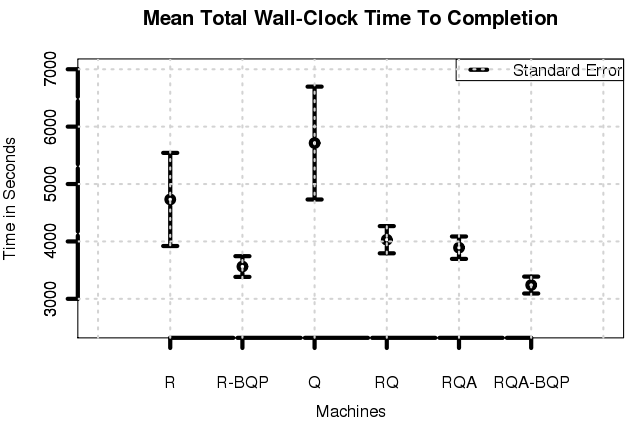
\includegraphics[scale=0.5]{./figures/Figure7.png}
\end{center}
\up\up\up\up\up\up\up\up\up
\caption{\tc for different configurations.  From Left to Right: (i)
  Ranger (ii) Ranger when using BQP, (iii) QueenBee, (iii) Ranger
  and QueenBee, (iv) Ranger, QueenBee and Abe, (v) Ranger, QueenBee 
  and Abe when using BQP.}
\label{fig:results}
\up\up\up\up\up\up
%\up\up\up\up\up\up
\end{figure}

In order to determine \tc using uncorrelated data, or more precisely less-correlated data, we repeat experiments ten times randomly interspersed over a period of few weeks.  We do this for three different machines on the TG -- Ranger, QueenBee and Abe.  Ranger is the flagship machine of the Texas Advanced Computing Centre; QueenBee (QB) the flagship machine of LONI and Abe a large machine at NCSA. Our results are plotted in Figure.~\ref{fig:results}.  As the results from the single-resource configuration show, the individual resources have somewhat different intrinsic performance.  Abe's performance is some where in between Ranger's and QueenBee's.  In general, the large fluctuations are due to fluctuations in the waiting times.
%This provides a measure of base-line performance. I

We then perform experiments using more than one computational resource on the TG. To be precise, we employ more than one computational resource towards the solution of a single instance of the problem.  Given that experiments are capable of utilizing three different TG resources, using two-resources at a time, gives us three different combinations. In Figure 9, we present data when Ranger and QueenBee are used collectively.  But, as a logical extension, we perform experiments wherein we utilize all three different TG resources. An important result that emerges is,
% that holds in general, but also for the specific instances investigated here, is that on average, 
that as the number of resources increases \tc decreases. This is demonstrated by the fact that, \tc (RQ) is lower than \tc (R) or \tc (Q).  Although \tc (RQA) is less than \tc (RQ), the change is less significant than when going from one to two resources; however, performing many more experiments should lead to a clearer distinction in \tcnsp.
% It is worth mentioning that the fluctuation in \tc (RQA) (as well as the mean) is higher than that for (R,Q) because of a single anamolous point in (R, Q, A).  
Finally, it is also important to point out that although \tc decreases, the overall number of CPU hours utilized does not increase. % This is a reconfirmation of the use of higher-level
% abstractions for enhanced performance.

In the next set of experiments, we employ BQP to autonomically decide which resources to utilize; we incorporate the decision making capability into the Lazarus framework.  R-BQP represents the scenario (Table 1), where BQP guides the selection of resource configuration on a predetermined machine (Ranger).  When using more than one machine, e.g., RQA-BQP, %represents the scenario where
both the selection of the resources and the selection of resource configuration are variables. For RQA-BQP, it is possible that even though three resources are available, all jobs be submitted to a single resource with much higher capacity or temporary lower load-factors (e.g, after a power-down/start-up). However, to correct for such corner cases and to take the more common case where all resources are essentially equal, we present data for RQA-BQP (Table 2) when all three resources are utilzed in the solution of the problem.

As shown in Figure.~\ref{fig:results}, the second data-point from the left, and the right-most data-point, indicate that the utilization of BQP to determine which resources and which resource configuration are used, leads to a drastic reduction in \tc compared to the simple case where Lazarus framework was used without autonomic behaviour. This is a powerful demonstration of the fact that even elementary autonomic behaviour can lead to significantly improved performance.

\begin{table}
\scalebox{0.775}{
\begin{tabular}{|c|c|c|c|c|}
\hline Sample \# & Machine & Queue & Num. Cores & Duration (hrs) \\ 
\hline 1-10& Ranger & normal & 64 & 2:00 \\ 
\hline 1-10& Ranger-BQP & development & 128 & 1:00 \\ 
\hline 
\end{tabular} 
}
\caption{Table showing the configurations chosen
  on Ranger, with and without BQP. Notice how the use
  of BQP has a small, but significant change in the queue, size and duration
  requested.}\up\up\up\up\up\up\up
\end{table}

This leads to the question, why does the use of autonomics result in
better performance figures? In a nutshell, the answer lies in the fact
that any decision relating to which resources to utilize is postponed
till run-time, which along with the capability to match better the
resource requirement to the resources available, leads to overall
performance enhancements. Specifically, as Tables I and II show, the
resource configurations -- number of cores assigned to a BigJob and
the queue duration requested, differ significantly between the
BQP-guided resource selection versus the unaided configuration.
Having established the power of autonomics in improving performance,
we now establish the mechanism behind the performance enhancement.

\up\up
\begin{table}
\scalebox{0.8}{
\begin{tabular}{|c|c|c|c|c|}
\hline \# of Samples & Machine & Queue & Num. Cores & Duration (hrs) \\ 
\hline 3 & Ranger     & development & 64  & 1:30 \\ 
\hline 5 & Ranger     & development & 64  & 2:00 \\ 
\hline 2 & Ranger     & development & 128 & 1:00 \\ 
\hline \hline 3 & QueenBee   & checkpt     & 16  & 2:00 \\ 
\hline 4 & QueenBee   & checkpt     & 16  & 1:00 \\
\hline 3 & QueenBee   & checkpt     & 32  & 1:00 \\ 
\hline \hline 3 & Abe        & dque        & 64  & 2:00 \\ 
\hline 7 & Abe        & dque        & 64  & 1:00 \\ 
\hline 
\end{tabular} 
}
\caption{Table showing  the selected configuration of the resources
  and the numer of times a particular configuration is chosen, when 
  the decision is guided by BzaQP. Data in this table corresponds to
  RQA-BQP; the experiments are repeated ten times. As can be seen, 
  the use of BQP results in a varying choice of resource  configuration on  different machines.  In contrast, when BQP is not used, a fixed configuration
  is employed.}\up\up\up\up\up\up
\end{table}

\jhanote{At some stage will have to elaborate on the following: (on all machines) for the BigJob size is always 64 with a duration fixed at 2:00 hours (although the chosen queue varies). So although there is not much change between different the BQP-guided runs, there is significant difference between BQP-guided and manual (unassisted) resource configurations}

\section{Challenges and Discussion}

The advantages of constantly running jobs on machines is the
development of an intuition to the state of the machine through
constant use. This is quantified in confidence numbers from
BQP. Interestingly enough, we could discern a higher chance of running
before deadlines during weekends than weekdays, and how some machines
favor larger jobs that have short durations and how other machines
favor the opposite. In general, different machines can have different
queuing policies and autonomic approaches such as those provided by
Lazarus can ``probe'' the queuing system to understand the non-public
policy and adapt accordingly.

A major issue in our use of the BQP is the choice of confidence and
quantile numbers. A detailed analysis is required to better assess our
choice of confidence and quantile numbers, and the impact these choices
make on overall performance.

Since we collected data from BQP without knowing it's granularity, we
tend to oversample the data. For example, if we sample BQP for jobs
lasting 1, 2 and 4 hours we might miss better configurations that last
3 hours. To avoid this incomplete and therefore misrepresentative
view, we mine BQP data at a fine grained level. This obviously leads
to a small (order of minutes) computational cost and is an issue that
needs to be addressed. Unfortunately, BQP results do not typically
vary at the level of granularity below 30 minutes.  The granularity
issue in BQP has two components: first, it is not known what the
refresh rate of the BQP data is (that is, how often it is collected
and analyzed; also this is not user-definable).  Secondly, the BQP's
sensitivity is also quite coarse-grained. For example, changing the
confidence level from 0.75 to 0.90 or to 0.60 typically did not
lead to different outputs.  Whether this is due to finite
time-sampling or other reasons is difficult to discern.

Perhaps the biggest challenge we encountered, and undoubtedly the most
frustrating, were the failures that went undetected, and lead us to
waste SUs, hours in the queue and of course hours waiting for results
that were corrupt. Many of these modes of failure can be solved using
a heart-beat from the actual simulation to a monitoring service that
allows the simulation to register its current state, current
iteration, progress rate, state of data, convergence data from the
solver etc. This will be implemented using the SAGA C++ API in Cactus
as a heartbeat thorn, and the monitoring service will be implemented
as a functionality in FAUST.  Similar failures, but
different machines and different solutions, thus there is a case to be
made that fault tolerance should be provided as a general-service.


\section{Future Work and Conclusion}

% \jhanote{Talk about forward and reverse scheduling/resource
%   reservation: normally we define a workload/requirement, and then
%   map that to the best available resource. Reverse scheduling is,
%   find the best resource/resource configuration and then adapt the
%   workload to the best resource/resource configuration. BQP based
%   autonomics, enables this to happen} Talk about forward and reverse
% scheduling and resource reservation:

In this paper we have demonstrated the very first beginnings of the
SAGA-based framework (Lazarus) that can be utilized by a broad range
of different applications to utilize Grids for autonomic computing.
Lazarus is distinct to other well established and successful
approaches such as Accord for autonomic computing, in that it is not a
component-based programming system but it is a framework already
composed of multiple components. Importantly the programming system
that is used is SAGA -- both for the application and the Lazarus
framework.

In addition to a clear performance advantage, the use of abstractions
based framework provides support for advanced features that would be
highly non-trivial to support otherwise.  For example, normally we
define a workload and/or a computational requirement and then map that
to the best available resource at that instant.  This is usually
referred to as {\it forward scheduling}.  An alternative approach
would be to first find the best resource and/or resource
configuration, and then adapt the workload to the best
resource/resource configuration; such an approach is often referred to
as {\it reverse scheduling}.  Thanks to a combination of BQP-based
autonomics (which enables the determination of the optimal resource)
along with the BigJob abstraction (which by decoupling the details of
the computational resources available from the computational
requirement provides the dynamic agility to utilize whatever resource
are made available) Lazarus is capable of supporting reverse
scheduling. This is a fine example of how the right abstractions can
be combined to support application-level requirements and provide
advanced functionality that might not be easily available otherwise.

We have captured the primary run-time characteristics of an
interesting and common class of applications and implemented a
solution to effectively manage this run-time complexity at the {\it
  application level}.  Our solution is perfectly acceptable as a
proof-of-concept, and modulo deployment and resource availability
issues, our approach will scale to problem sizes encountered in the
many science and engineering problems.  Lazarus in its current
incarnation will be used by other applications. Specifically, in
addition to Ensemble Kalman filters %~\cite{DataAssim, KalmanPaper},
that we investigate here -- there are several other classes of
applications ---``first principles'' Grid applications such as
GridSAT~\cite{gridsat03} and applications which based upon resource
aware ``learning'' algorithms~\cite{ majority_voting}, for which it is
both difficult to estimate precisely the resource requirements while
explicitly needing to marshal the distributed resources and thus can
benefit greatly from autonomic approaches. We will in the future
utilize, and extend capabilities of the the Lazarus framework to
support additional computational science and engineering applications.

By working to interface and support several different types of
applications, ultimately we aim to work towards a general purpose
approach to support high-level formulation of strategy and its
translation into specific mechanism and parameters to support
autonomic behaviour.

And although Lazarus in its current incarnation can support multiple applications and application classes, there is scope for additional developments and increased sophisticated capabilities within Lazarus.  Specifically, Lazarus will evolve to utilize more sophisticated Information Services -- but this is currently restricted by the lack of widespread availability of information services. Last but not least, Lazarus in of itself will utilize other specialized frameworks -- such as FAUST~\cite{faust_url}.

One of the planned extensions to Lazarus is the addition of adaptive
queuing systems. As it stands, Lazarus will submit optimized BigJobs
to resources and wait for them to get through the queue, run and
terminate.  When the number and size of subjobs is sufficiently large
and the resources considerably congested, there will be a considerable
amount of time during which larger, less congested resources may have
come online or better BQP BigJob configurations have emerged; all of
this while the original BigJobs have not started to run. A BigJob can
then be scheduled on a new resource or another BigJob of different
size and duration can be submitted to the queue and existing BigJobs
that are in the queue can be deleted.  Such adaptive scheduling will
be implemented in the Lazarus framework using the upcoming FAUST
framework.

One of the proposed features of the FAUST framework that we will be making extensive use of is the heartbeat monitor. This consists of a client-side service that is called from the actual simulation and a server-side service that is called from Lazarus. The client-side service, effectively a library function, will update the SAGA advert database entry of that particular simulation with vital information and statistics, including the current iteration, the amount of memory allocated, the convergence rate and so on. The current design allows for the application to register a key-value pair of entries to the advert database, making it flexible and application independent. The server-side service is called by Lazarus to check on the status of running simulations, make sure the allocated memory is within tolerance, the convergence rate is acceptable and the time elapsed between iterations does not vary greatly between simulations. 

% dynamically adapt mechanisms, and We created a single set of Globus
% adaptors and deployed them on distinct Grids. Our application
% successfully utilized these adaptors, without any further
% customization, which goes to show that

%We also discussed how the deployment of this model application across
%two distinct Grids was trivial as it only required the deployment of
%of the appropriate SAGA adaptors.  

% There are many applications that need to use federated
% Grids~\cite{clade06, gin_paper}.  Utilizing SAGA to develop, or at
% least provide Grid-functionality is a useful strategy. Therefore, if
% the development and deployment of applications across federated grids
% is to be facilitated, SAGA adaptor activity -- development and
% deployment, needs to be self-sustaining and thus requires explicit
% support, from both the middleware developers and resource providers.

% The success of e-Science critically depends upon the availability of
% e-Infrastructure.  But the promise of e-Science will be hollow without
% delivery of the applications and application-enabling paradigms and
% technology that can effectively utilize this new infrastructure. We
% believe SAGA is an important first step in this direction.

\section{Acknowledgments}
We acknowledge Andre Luckow, who should have been an author on this
paper, had it not been for bureaucratic hurdles.  SJ acknowledges UK
EPSRC grant number GR/D0766171/1 for supporting SAGA and the e-Science
Institute, Edinburgh for the research theme, ``Distributed Programming
Abstractions'' and participants in the theme. SJ also acknowledges
financial support from NSF-Cybertools and NIH-INBRE Grants. YE
acknowledges the Department of Energy and Louisiana Board of Regents
(award No. DE-FG02- 04ER46136) for providing funding and support. YE
would like to acknowledge Prof. Chris White, Prof. Mayank Tyagi and
Dr. Xin Li and useful discussions with Ole Weidner. This work would
not have been possible without the efforts and support of other
members of the SAGA team. The authors acknowledge the Texas Advanced
Computing Center (TACC) at The University of Texas at Austin, LONI, CCT and
NCSA for providing HPC resources that have contributed to the research
results reported within this paper.

\bibliographystyle{IEEEtran} 
\bibliography{saga_tg08}
\end{document}

Another abstraction
-- the SAGA Glide-In abstraction is used to support the commonly
occurring requirement to schedule multiple sub-tasks relative to each
other and not in competition with other jobs submitted to the batch
queue system.  Thus, a \texttt{big\_job} and \texttt{sub\_job} object
are defined; for each \texttt{big\_job} object, a Glide-In job with
the desired number of resources is started, and \texttt{sub\_job}
objects -- which correspond to individual replicas, are mapped to a
\texttt{big\_job} using the jobid as reference. It is helpful to
reiterate that although there is a big\_job object, it is submitted
as a Glide-In job, and that BigJob abstraction in turn utilises the
Glide-In abstraction to map the individual big-job and sub-jobs to
physical resources.

Figure~\ref{fig:abstractions} summarizes the abstractions developed
and used in this work to support the clustering of sub-jobs into a
larger big-jobs and the effective dispatching of the sub-jobs.  The
specific capability to cluster sub-jobs, is provided to the
application via the \emph{BigJob} abstraction. This abstraction
enhances the SAGA job model \jhanote{Need a sentence or two about what
  ``enhancing the SAGA job model'' means, ie in turn outlining what
  the SAGA Job Model is?}  with the capability to allocate
larger chunks of resource for a single job.
% allocate larger chunks of resources prior to an application run.
\jhanote{AndreL: Not sure what the commented out line was about.. if
  you'd like to reinstate, please clarify/elaborate}
